\documentclass{article}\usepackage[]{graphicx}\usepackage[]{color}
%% maxwidth is the original width if it is less than linewidth
%% otherwise use linewidth (to make sure the graphics do not exceed the margin)
\makeatletter
\def\maxwidth{ %
  \ifdim\Gin@nat@width>\linewidth
    \linewidth
  \else
    \Gin@nat@width
  \fi
}
\makeatother

\definecolor{fgcolor}{rgb}{0.345, 0.345, 0.345}
\newcommand{\hlnum}[1]{\textcolor[rgb]{0.686,0.059,0.569}{#1}}%
\newcommand{\hlstr}[1]{\textcolor[rgb]{0.192,0.494,0.8}{#1}}%
\newcommand{\hlcom}[1]{\textcolor[rgb]{0.678,0.584,0.686}{\textit{#1}}}%
\newcommand{\hlopt}[1]{\textcolor[rgb]{0,0,0}{#1}}%
\newcommand{\hlstd}[1]{\textcolor[rgb]{0.345,0.345,0.345}{#1}}%
\newcommand{\hlkwa}[1]{\textcolor[rgb]{0.161,0.373,0.58}{\textbf{#1}}}%
\newcommand{\hlkwb}[1]{\textcolor[rgb]{0.69,0.353,0.396}{#1}}%
\newcommand{\hlkwc}[1]{\textcolor[rgb]{0.333,0.667,0.333}{#1}}%
\newcommand{\hlkwd}[1]{\textcolor[rgb]{0.737,0.353,0.396}{\textbf{#1}}}%

\usepackage{framed}
\makeatletter
\newenvironment{kframe}{%
 \def\at@end@of@kframe{}%
 \ifinner\ifhmode%
  \def\at@end@of@kframe{\end{minipage}}%
  \begin{minipage}{\columnwidth}%
 \fi\fi%
 \def\FrameCommand##1{\hskip\@totalleftmargin \hskip-\fboxsep
 \colorbox{shadecolor}{##1}\hskip-\fboxsep
     % There is no \\@totalrightmargin, so:
     \hskip-\linewidth \hskip-\@totalleftmargin \hskip\columnwidth}%
 \MakeFramed {\advance\hsize-\width
   \@totalleftmargin\z@ \linewidth\hsize
   \@setminipage}}%
 {\par\unskip\endMakeFramed%
 \at@end@of@kframe}
\makeatother

\definecolor{shadecolor}{rgb}{.97, .97, .97}
\definecolor{messagecolor}{rgb}{0, 0, 0}
\definecolor{warningcolor}{rgb}{1, 0, 1}
\definecolor{errorcolor}{rgb}{1, 0, 0}
\newenvironment{knitrout}{}{} % an empty environment to be redefined in TeX

\usepackage{alltt}

\usepackage{amsmath, amssymb}
\usepackage{graphicx}
\usepackage{hyperref}
\IfFileExists{upquote.sty}{\usepackage{upquote}}{}
\begin{document}

\title{Pol Sci 630:  Problem Set 8: Dummy Variables and Interactions (Part 2)}

\author{Prepared by: Anh Le (\href{mailto:anh.le@duke.edu}{anh.le@duke.edu})}

\date{Due Date: Tue, Oct 20, 2015, 10 AM (Beginning of Lab)}

\maketitle

\section{Interaction (8 points)}

\subsection*{a)}

Download FDI, tariff, and GDP data from WDI for all countries, year 2010 (\verb`indicator = c("BX.KLT.DINV.CD.WD", "TM.TAX.MRCH.SM.AR.ZS", "NY.GDP.MKTP.CD")`). Clean the data as usual. Run the following regression, showing a stargazer result table.

\begin{align}
\log(FDI) &= \beta_0 + \beta_1 tariff + \beta_2 \log(gdp) + \beta_3 tariff \times \log(gdp)
\end{align}

\subsection*{b)}

Mathematically, what is the marginal effect of tariff on logfdi (i.e. taking partial derivative with regards to tariff)? (Hint: This would be a function of loggdp)

Plugging in the number, what's the marginal effect of tariff on logfdi, holding loggdp at its median value? Note: Use \verb`\Sexpr()` to extract coefficients from the model, do not hand write your calculation.

\subsection*{c)}

Using \verb`ggplot2`, plot the marginal effect of tariff on logfdi (y-axis) against different values of loggdp (x-axis). (Hint: Create a data frame, in which one variable is the values of loggdp, the other variable is the corresponding marginal effect given that value of loggdp. This data frame is the data that makes up your plot. The plot is just a line.)

\subsection*{d)}

With log fdi on the y-axis, tariff on the x-axis, plot the effect of tariff on log fdi when log gdp is at the 25\%, 50\%, and 75\% percentile. Brownie point if you do this in ggplot2.

(Hint: The plot should have 3 lines, each according to a value of log gdp. This is the plot you saw in last lab, with confidence interval included)

\subsection*{e) Interpretation}

Interpret the result (i.e. statistical significance and effect size) using information from both the table and the two plots.

\section{ggplot2 (4 points)}

Plot this. Note: DO NOT look at the .Rnw code that generates the plot.

If you did try but couldn't figure out, you can look at the code for hints, but then you have to add comments to explain what the code does.

\begin{knitrout}
\definecolor{shadecolor}{rgb}{0.969, 0.969, 0.969}\color{fgcolor}
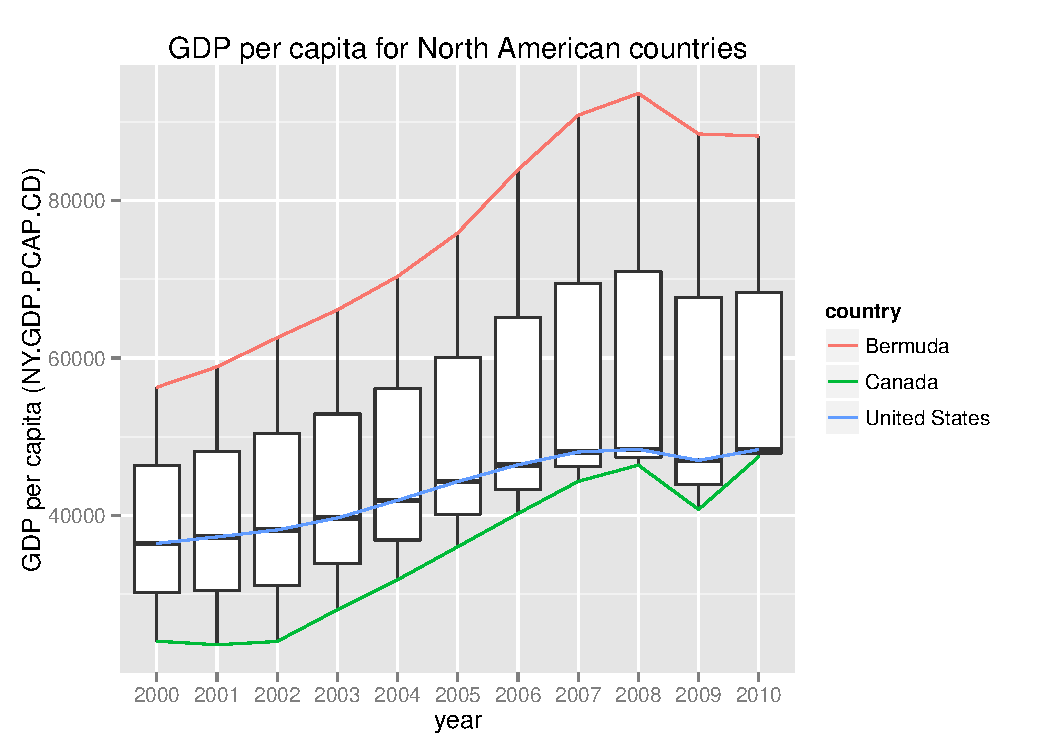
\includegraphics[width=\maxwidth]{figure/unnamed-chunk-1-1} 

\end{knitrout}

\section{ANOVA (4 points)}

\subsection*{a)}

Load the diamond dataset in R (\verb`data(diamonds)). With \verb`price` as the dependent variable, run 1) one-way ANOVA on \verb`cut`; 2) two-way ANOVA on \verb`cut` and \verb`clarity` and their interaction.

Interpret the table (i.e. which factor is important in determining the diamond's price?)

\subsection*{b)}

What is the expected price for a diamond that has:
\begin{itemize}
\item Ideal cut, VS1 clarity
\item Very Good cut, VVS1 clarity
\end{itemize}

Note: You'll have to do dummy regression like last homework, not ANOVA. Also you need to remove the order from the factors \verb`cut` and \verb`clarity`. See \href{http://stackoverflow.com/questions/17592524/how-to-remove-ordering-of-the-levels-from-factor-variable-in-r}{this SO answer}. Remember to use \verb`\Sexpr{}`, don't write down answers by hand (see how I use \verb`\Sexpr{}` from last solution if confused.)

\end{document}
